\section[DFT Settings]{Selected DFT Code, Pseudopotentials and Parameters}


\subsection{Quantum Espresso}

There are a choice of several different \acrshort{dft} programs to choose from, including VASP, Siesta and Quantum Espresso.  The open source Quantum Espresso includes the PWscf binary that solves electronic structure calculations with plane wave pseudopotentials.  It calculates the total energy of a system as well as the forces between atoms and the stress on the simulation box.  

As the calculations contain Iron, it is important to take into account the magnetism caused by the filling of the d-shell.  PWscf gives three modes: non-magnetic, collinear spin and non-collinear spin.  



\subsection{Pseudopotential Selection}

The pseudopotentials were downloaded from the Quantum Espresso PSLibrary with url:

http://www.quantum-espresso.org/pseudopotentials/pslibrary 

There are several categories of pseudopotential available.  The pseudopotentials may be fully relativistic or not.  The DFT calculations in this work will be non-spin or collinear spin and the element with the largest number of electrons will be Palladium, with electrons in the s, p, d shells.  There will be no elements used in this work with f shell electrons, so a non-relativistic pseudopotential will be used for each element.

There are a number of choices of exchange-correlation functional, depending on the element:

\begin{itemize}
\item pz: Perdew-Zunger (LDA)
\item vwn: Vosko-Wilk-Nusair (LDA)
\item pbe: Perdew-Burke-Ernzerhof (GGA)
\item blyp: Becke-Lee-Yang-Parr (BLYP)
\item pw91: Perdew-Wang 91 gradient-corrected 
\end{itemize}

In the literature, LDA and BLYP are used for organic DFT calculations.  LDA and GGA type pseudopotentials have been used to model solids and, in particular, the GGA type have been used to study metals as they are more reliable at calculating parameters such as $a_0$ (see section \ref{section:ggavslsda}).  Several elements were tested to compare the results of LDA and GGA pseudopotentials to the experimental values for the lattice parameter of each.

The settings used were:

\begin{itemize}
\item ecutwfc: 71 
\item ecutrho: 430 
\item k-points: 9 9 9 Monhurst-Pack grid offset
\item smearing: 0.04 Ry Mazari-Vanderbilt cold smearing
\item calculation type: non-polarised calculation
\item pseudopotentials: PZ for LDA, PBE for GGA
\end{itemize}

The results were computed as follows:

\begin{table}[h]
\begin{center}
\begin{tabular}{c c c c c}
\hline\hline
Element & Crystal & $a_0$ exp. (ang) & $a_0$ LDA (ang) & $a_0$ GGA (ang) \\
\hline\hline
Al     & FCC  &  4.05  &  3.98  &  4.04   \\ 
Fe     & BCC  &  2.87  &  2.69  &  2.75   \\ 
Pd     & FCC  &  3.89  &  3.84  &  3.93   \\ 
Cu     & FCC  &  3.61  &  3.49  &  3.59   \\ 
\hline\hline
\end{tabular}
\end{center}
\caption{Predicted lattice parameters based on the density, atomic number and type of structure}
\label{table:computedlattice}
\end{table}

The simpler LDA pseudopotentials consistently underestimate the lattice parameter $a_0$ for the four metals tested, and on average they underestimate by 3\%.  The GGA calculations are within 1.5\% of the experimental value.


\subsection{Smearing Type}

The material being studied here is a metal/metal alloy, and this has important consquences when setting up the calculation.  The conduction and valence bands overlap in a metal, and the fermi energy passes through this overlap. When the occupied states are summed, integrating over all k-points k\cite{marzarivanderbilt}, those bands that cross the Fermi energy will drop to zero.  There are two solutions used here to reduce this abrupt drop off: increase the number of k-points, or add a smearing to smooth the occupation function.  Previous work has given the following suggested smearing types and values as a start point.

\begin{itemize}
\item Degauss values 0.01Ry Methessel-Paxton \cite{AdsorptionBR2}
\item Fermi-Dirac 0.01eV (0.00074Ry) \cite{NaDiffusion}
\item Marzari-Vanderbilt 0.01Ry \cite{ScBiandYBi}
\item Degauss 0.03 + 0.05 \cite{CuandPd}
\item Marzari-Vanderbilt 0.05Ry \cite{ecHeuslerAlloy}
\end{itemize}

This suggests that a range between 0.01Ry to 0.05Ry should be investigated as a sensible range of smearing energies.  There are a choice of four smearing functions in QuantumEspresso.

\begin{itemize}
\item Gaussian
\item Fermi-Dirac
\item Methfessel-Paxton
\item Marzari-Vanderbilt
\end{itemize}

Functions such as the Gaussian and Fermi-Dirac are not cold smearing, and will converge to the wrong energy whereas the Mazari-Vanderbilt and Methfessel-Paxton are designed to reduce and heating whilst smearing the electron wavefunction.  An author of QuantumEspresso, N. Marzari, co-developed the cold smearing Marzari-Vanderbilt function, and this was selected as it had appeared a number of times in the literature and throughout the QuantumEspresso tutorials.  






\subsection{Parameter Convergence}

The energy cutoff, charge density, k-point and smearing values must be selected carefully for any similar DFT calculation.  There is a balancing act between the accuracy of the result of a particular calculation and computational time.  This will also vary with the pseudopotential, complexity of the electron configuration of the atoms, whether or not the calculation is with or without spin, and so on.

The pseudopotentials and smearing type have already been selected, and the first set of calculations will not include magnetism.  The parameters must work well with high symmetry geometries, such as a BCC or FCC crystal with the atoms in their exact position, but also where the atoms have been slightly perturbed from their exact position in the lattice.

\subsubsection{Ecutwfc and Ecutrho}

A primitive FCC or BCC is created and the atoms are slightly perturbed, breaking symmetry but also putting forces on each atom within the cell.  A reasonably high number of k-points are used and the smearing value should be low, but the k-point values in particular will depend upon the computing resources you have available.

Pick a low ecutwfc and set the ecutrho equal to four times the value of the ecutwfc.  Depending on the pseudopotential, the calculation may fail because the values are too small.  If this is the case, continue increasing the value in small (perhaps 5Ry) increments until the calculation runs successfully.

Next, continue to increase the ecutwfc value whilst increasing the value of ecutrho such that $ecutrho = 4 \times ecutwfc$ in steady increments (5Ry).  Once the calculated force and energy per 1Ry increment fall below a threshold set by the user, the values have converged.  In this work, the convergence values were:

\begin{itemize}
\item Energy convergence per 1Ry: $1.0 \times 10^{-6}$ Ry ($1.36 \times 10^{-5}$ eV)
\item Force convergence per 1Ry: $1.0 \times 10^{-5}$ Ry/Bohr ($2.57 \times 10^{-4}$ eV/Ang)
\end{itemize}

At this point, it may be possible to reduce the ecutrho value further while remaining within this convergence threshold, so the ecutwfc value is held fixed while the ecutrho value is reduced in steps of 5Ry.

Finally, attempt to reduce the value of ecutwfc further in 1Ry steps while holding the ecutrho value steady for as long as the convergence value remains within the set threshold.

\subsubsection{K-Points and Smearing Value}

A configuration with a similar size and number of atoms as those in the calculations should be created.  In this work, the reference database and bulk properties will be calculated using 32 atom configurations in an approximately sized $7 \times 7 \times 7$ angstrom box.  The Iron FCC k-points and smearing are calculated using a 32 atom FCC box with sides length 7.2 angstrom and the Palladium with a 32 atom FCC box with sides length 7.8 angstrom.

As with the ecutwfc and ecutrho convergence calculations, the atoms are slightly perturbed from their exact crystal positions, putting a force on the atoms and breaking the symmetry (as will be the case for the configurations used for fitting). 

The convergence process is more complex for k-points and smearing.  There might be a convergence that, at face value, looks better (a smaller convergence value and a decrease in the computation time and memory requirements) for combinations with a higher smearing value, but it is preferred to have a smaller smearing value with a higher number of k-points, while maintaining a reasonable computing time, as the greater the smearing the further the calculated value is from the actual calculated value (with no smearing and a very high number of k-points).

A 2D plot of energy and force values as a function of number of k-points and smearing may then be used to choose reasonable settings that balance the requirements.







\FloatBarrier
\subsection{QECONVERGE Python Code}
\label{code:qeconverge}

The process requires the creation of many input files, and manually editing these files is time consuming and vulnerable to human error. Over 100 input files may be required to converge the ecutwfc and ecutrho values, with a further 50-100 required to generate the 2D k-point and smearing plots.  A python code, QECONVERGE, was developed to automate this process and plot the results automatically for the user (section \ref{code:qeconverge}).

The program reads an input file into memory, and this contains the settings for the convergence run.  A template PWscf input file is also loaded, and this will detail any required PWscf settings, such as the pseudopotentials, atom species and so on.  

Once these files have been loaded, the first stage of the program runs to determine the ecutwfc and ecutrho values that are within the force and energy convergence thresholds provided by the user.  The program creates a crystal based on the settings, for example an FCC, BCC or SC crystal supercell.  The exact atomic positions are likely to be the optimal, relaxed, positions and so the overall forces on each atom will be zero.  The program randomly varies the atomic positions, and this results in a configuration with forces between the atoms.

The wfc value starts with the user defined ecutwfc starting value, and this is increased until the change in energy and force both converge to within the specified thresholds.  The ecutrho value is increased simultaneously, and is four times the ecutwfc value.  In the second stage, the ecutrho value is decreased and the ecutwfc value is fixed while the energy and force remain within their respective convergence thresholds.  Finally, the program attempts to decrease the ecutwfc value further.

Following the energy and charge density cutoff, the program then runs a number of calculations in order to produce a collection of colour density plots of energy cutoff vs density cutoff, plotting the convergence of total energy and total force.  This allows the user to visualise the convergence surface and select cutoff values manually, if desired.

The final part of the program is to help the user decide upon degauss and k-point values.  The converged ecutwfc and ecutrho values from the first part of the code are used, and the k-point start, end and increment amounts are set by the user, as is a list of smearing degauss values.  2D colour plots of force and energy convergence as smearing changes and k-point value changes are prepared and saved so the user may study these to determine the best combination for their application.

The randomised atom positions use a seed that may be set in the input file.  This means that, although they are pseudo-rng generated, they are repeatable given the same random seed.  Every successful PWscf calculation is logged and saved.  If the program runs multiple times, the cached output files are used rather than recalculating every input file.

The source code and instructions on how to use the program are available to download from GitHub.

https://github.com/BenPalmer1983/qeconverge












\FloatBarrier
\subsection[DFT Parameter Convergence]{Convergence of Key DFT Settings and Testing}

Prior to generating a database of atom configurations, calculated forces, stresses and energies, key \acrshort{dft} settings needed to be selected and tested.  The Python code QECONVERGE was written then used to converge the ecutwfc, ecutrho, k-points and degauss smearing values for each of the pseudopotentials required.
  
As discussed in previously (section \ref{section:backgroundpseudopotentials}) the \acrshort{gga} type pseudo-potential more reliably calculated the bulk properties of a material when compared to \acrshort{lda}/\acrshort{lsda}, and a copy of the earlier table is given in table \ref{table:ggavslsdacopy}.

\FloatBarrier 
\begin{table}[h]
\begin{center}
\renewcommand{\arraystretch}{1.2}
\begin{tabular}{c c c c}
\hline\hline
Pseudo-potential & Element & a/angs & $B_0$/GPa \\
\hline\hline
Experimental    & Na      & 4.29\cite{periodictablena} & 6.3\cite{periodictablena} \\
Na.pz-spn-kjpaw\_psl.1.0.0 & Na & 4.06 & 8.72 \\
Na.pbe-spn-kjpaw\_psl.1.0.0 & Na & 4.20 & 7.67 \\
Na.pbesol-spn-kjpaw\_psl.1.0.0 & Na & 4.17 & 7.50 \\
Experimental    & Al      & 4.05\cite{periodictableal} & 76\cite{periodictableal} \\
Al.pz-nl-kjpaw\_psl.1.0.0 & Al & 3.98 & 78.6 \\
Al.pz-n-kjpaw\_psl.1.0.0 & Al & 3.98 & 78.6 \\
Al.pbe-nl-kjpaw\_psl.1.0.0 & Al & 4.04 & 91.3 \\
Al.pbe-n-kjpaw\_psl.1.0.0 & Al & 4.04 & 75.0 \\
Al.pbesol-nl-kjpaw\_psl.1.0.0 & Al & 4.01 & 87.7 \\
Al.pbesol-n-kjpaw\_psl.1.0.0 & Al & 4.01 & 79.0 \\
\hline\hline
\end{tabular}
\end{center}
\caption{Experimental vs \acrshort{lsda} vs \acrshort{gga} - the \acrshort{dft} values were computed with a PWscf\cite{quantumespresso} using a 2x2x2 cell, 7x7x7 kpoints and ecutwfc=50}
\label{table:ggavslsdacopy}
\end{table}

\FloatBarrier 

The following pseudo-potential files were used for each element:

\begin{itemize}
\item Aluminium: a plane wave GGA potential Pd.pbe-spn-kjpaw\_psl.1.0.0.UPF
\item Chromium: a plane wave GGA potential Cr.pbe-spn-kjpaw\_psl.1.0.0.UPF
\item Iron: a plane wave GGA potential Fe.pbe-spn-kjpaw\_psl.1.0.0.UPF 
\item Palladium: a plane wave GGA potential Pd.pbe-spn-kjpaw\_psl.1.0.0.UPF
\item Ruthenium: a plane wave GGA potential Ru.pbe-spn-kjpaw\_psl.1.0.0.UPF
\end{itemize}

For each pseudo-potential, the ecutwfc, ecutrho and kpoint and degauss settings were converged.  Ideally, the k-points settings would have been increased, but doing so would have been prohibitive due to the amount of time taken to perform each calculation.

By the time calculations were being executed for a 32 atom supercell, one node of 20 processor cores would run for several days up to a week or more, requiring the calculation to be submitted to the job queue multiple times.  Al is also considered in the results section, as it is a simpler atom to run trial calculations with, and to compare to experimental results.

The relaxed crystal lattice parameters were calculated for Fe, Cr, Pd and Ru.  Cr will not be used in either the Fe-Pd or Fe-Ru fitting calculations.  However, there is a large increase in computation time between non-spin and collinear spin calculations.  The ferromagnetic structure of BCC Fe, antiferromagnetic structure of FCC Fe and BCC Cr were investigated. 

\FloatBarrier
\begin{figure}[h]
\begin{center}
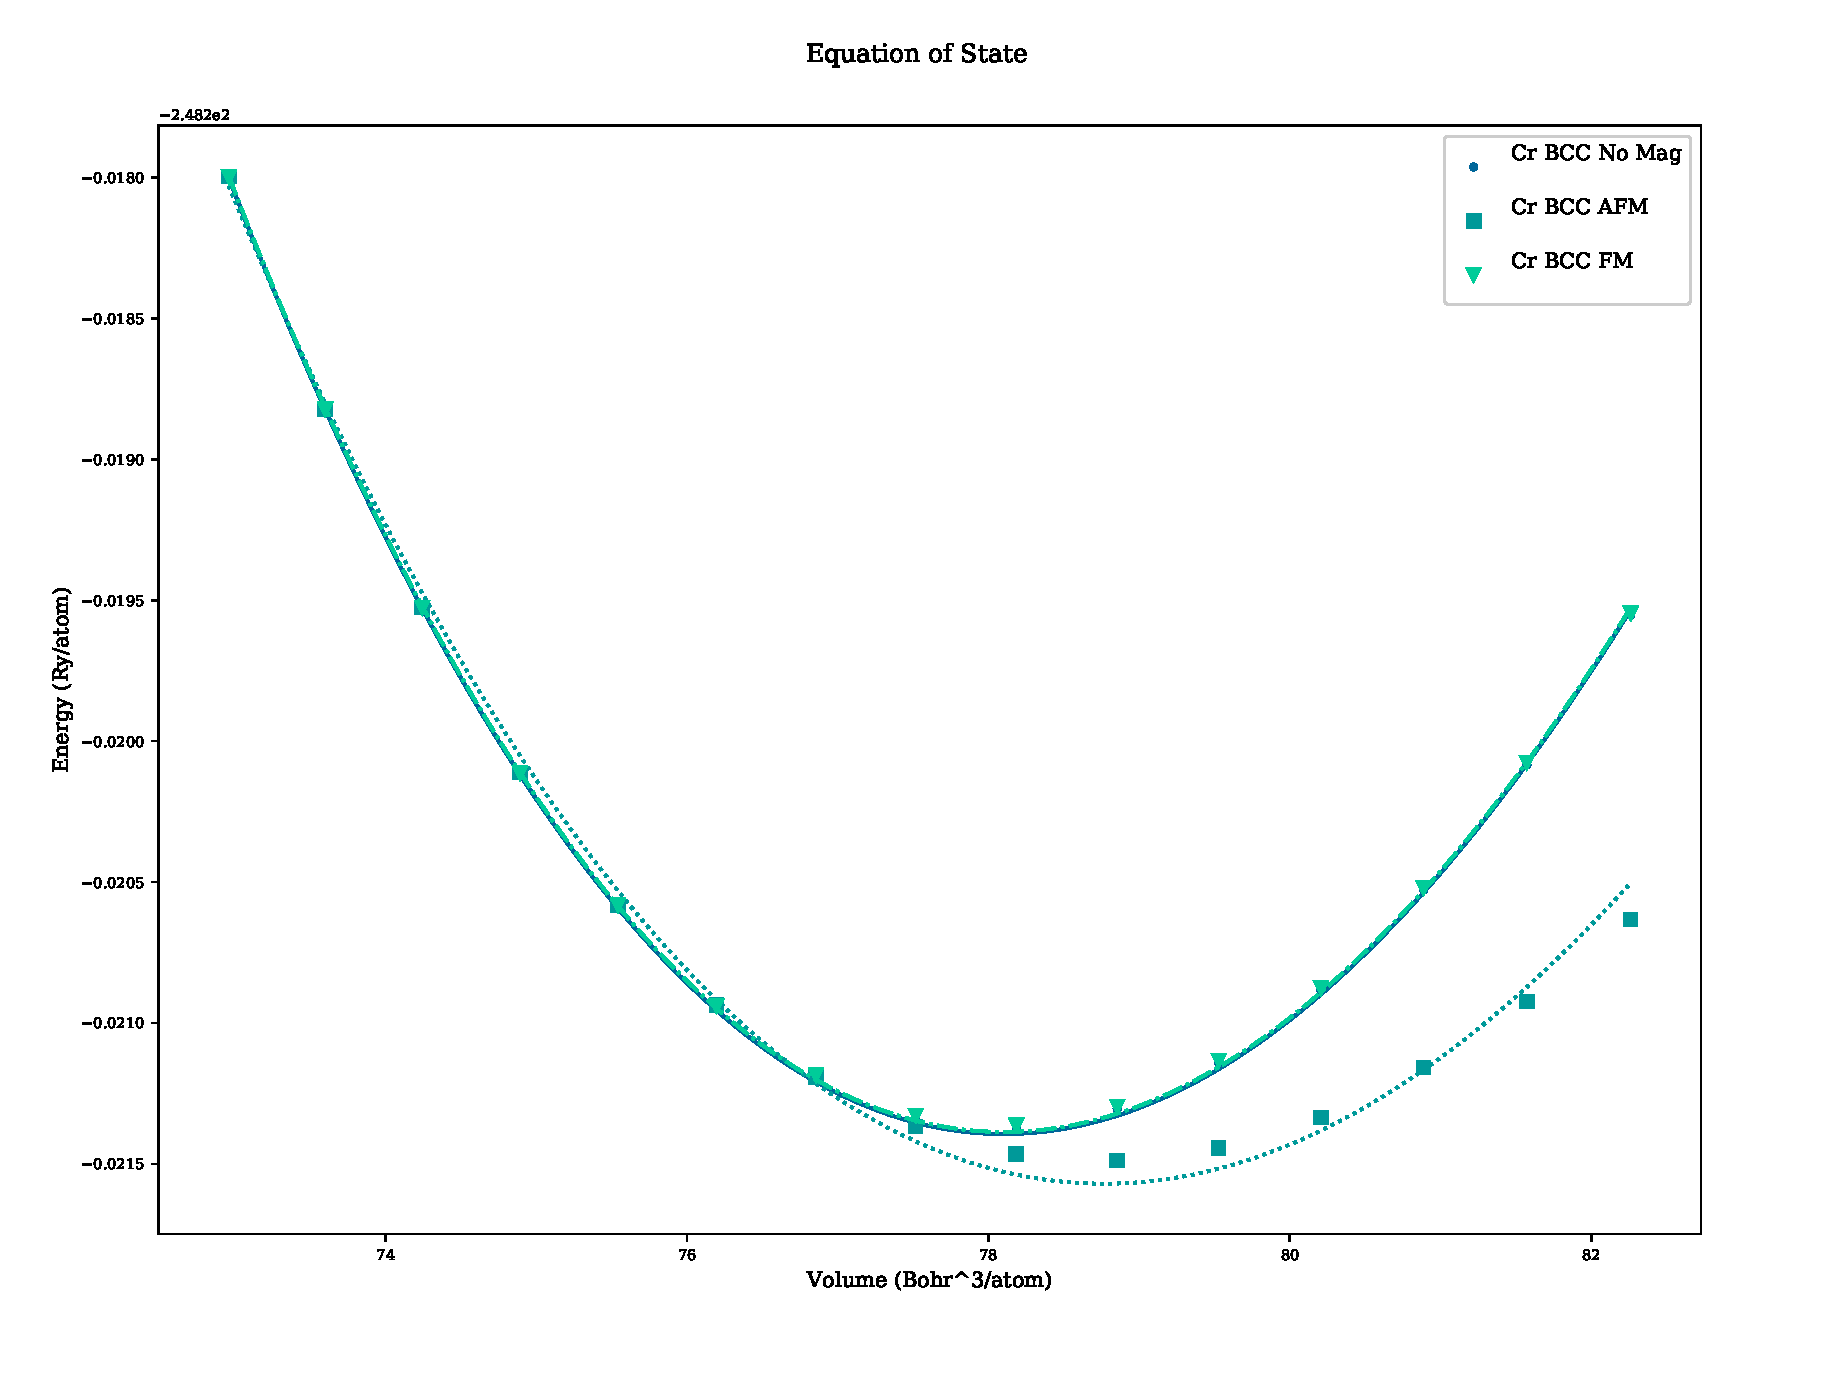
\includegraphics[scale=0.45]{chapters/potentials_fe_pd_ru/qeeos_plots/cr-mag/eos.eps}
\caption{Equation of state fit through data points for Chromium BCC with no magnetism, ferromagnetic and antiferromagnetic configurations}
\label{fig:chromiumeos}
\end{center}
\end{figure}


\FloatBarrier
\begin{table}[h]
\begin{center}
\renewcommand{\arraystretch}{1.2}
\begin{tabular}{c c c c c c}
\hline\hline
Description & $A_0$ (ang) & $V_0$ (bohr3) & $B_0$ (GPA) & $E_0$ (Ry) (DFT Only) \\
\hline\hline
Exp. & 2.91 & 83.23 & 160 & - \\
AFM & 2.86 & 78.77 & 217 & -248.2216 \\
FM & 2.85 & 78.10 & 267 & -248.2214 \\
No Mag & 2.85 & 78.102 & 267 & -248.2214 \\
\hline\hline
\end{tabular}
\end{center}
\caption{Chromium properties with and without collinear spin}
\label{table:crproperties}
\end{table}
\FloatBarrier

The equation of state was calculated for Chromium BCC in three ways: (1) with magnetism switched off, (2) atoms set in a ferromagnetic configuration (collinear, all in the same direction), (3) atoms set in an antiferromagnetic configuration (collinear, atoms in the same cell with spin in opposing directions).  

The DFT calculated values for the bulk modulus were larger than expected, but the antiferromagnetic calculation was much closer to the experimental value (table \ref{table:crproperties}).  The $E_0$ values do not reflect the actual energies, but show the relative calculated values.  The antiferromagnetic configuration gives the lowest, optimum, energy (fig. \ref{fig:chromiumeos}).

\FloatBarrier
\begin{figure}[h]
\begin{center}
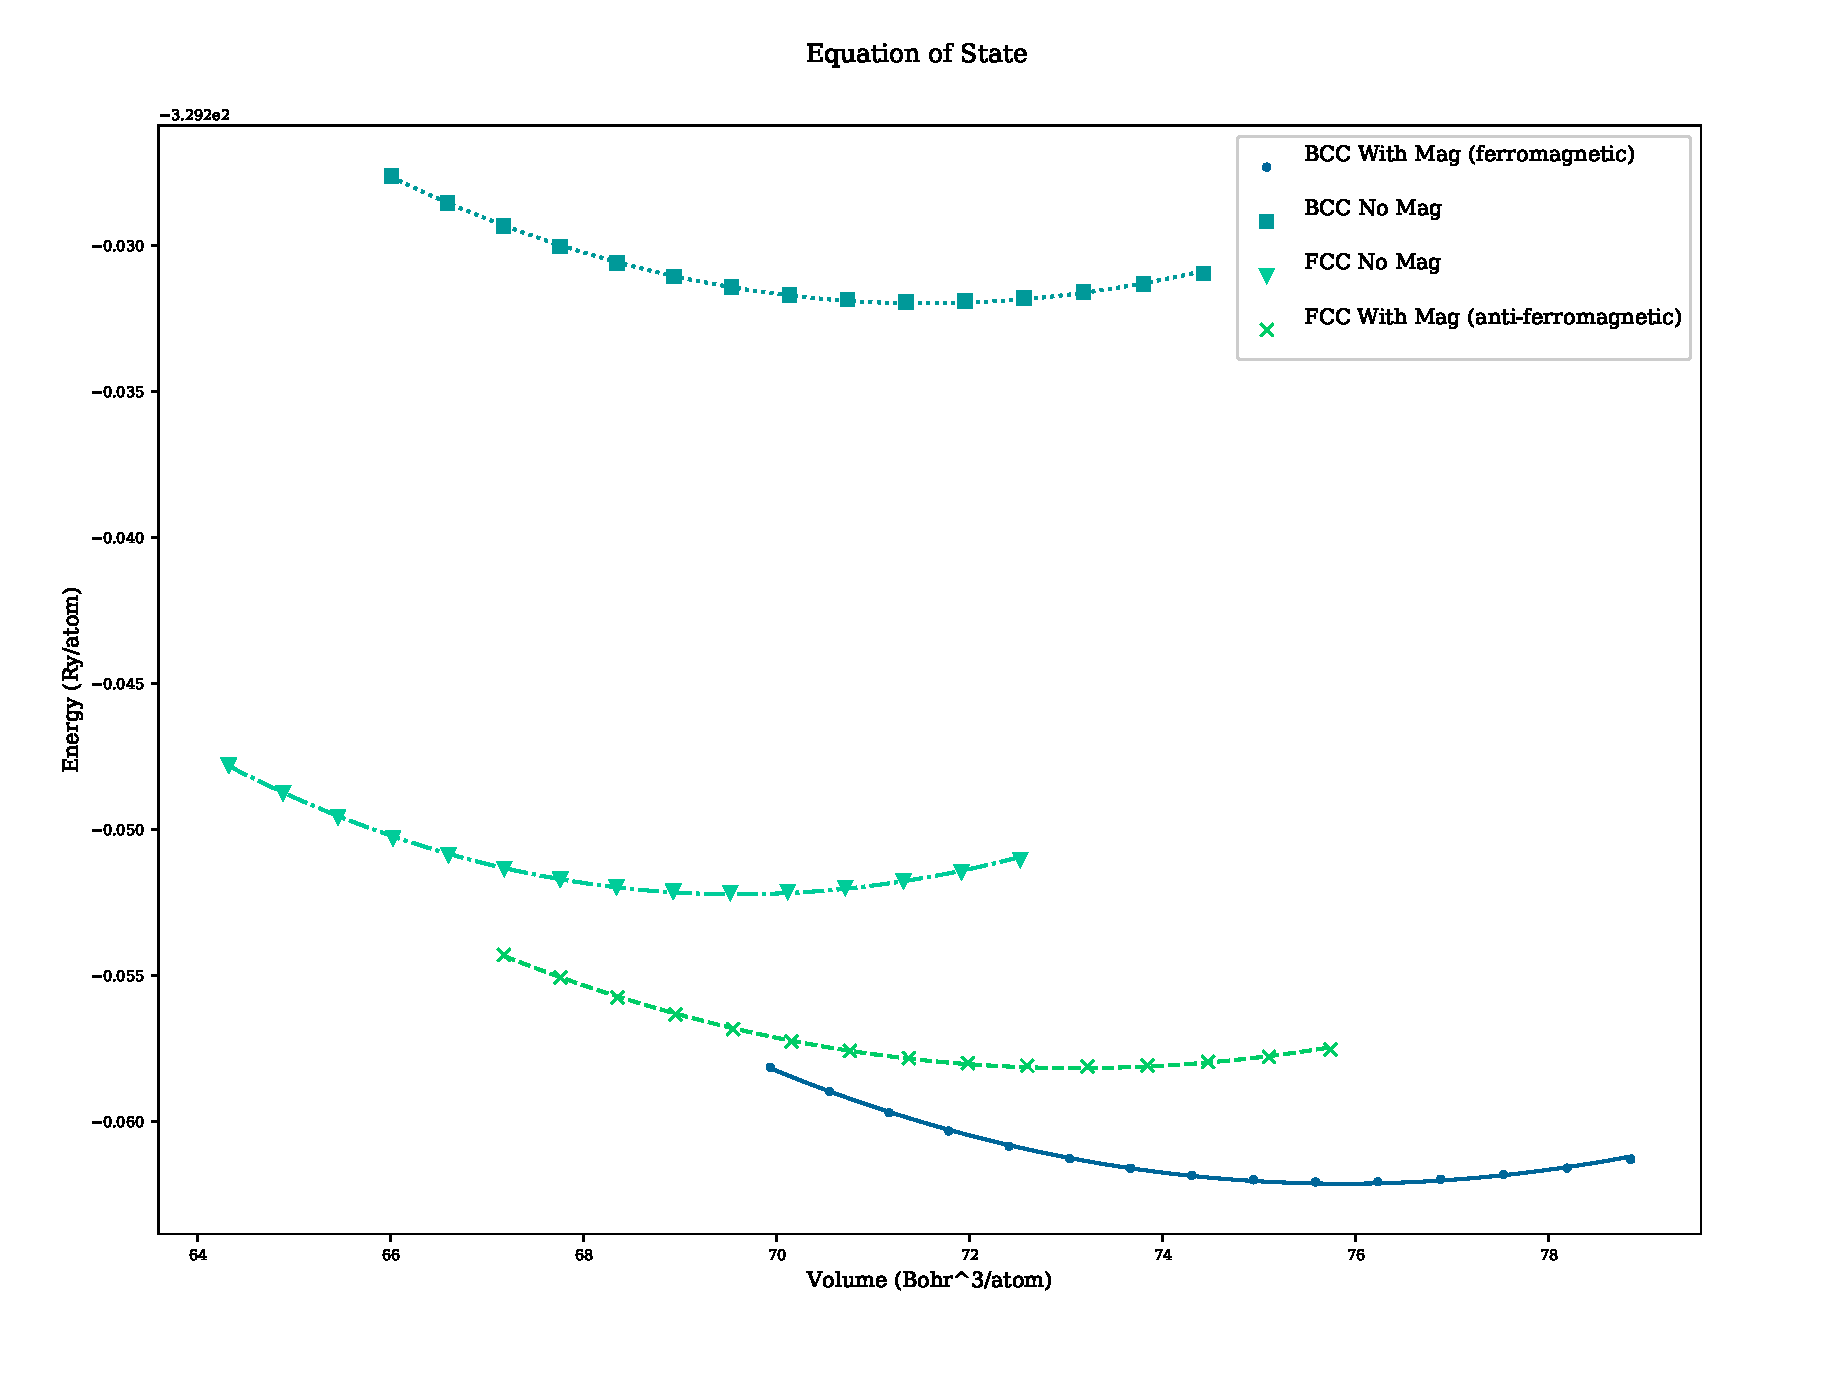
\includegraphics[scale=0.45]{chapters/potentials_fe_pd_ru/qeeos_plots/fe-mag/iron_eos_comparison.eps}
\caption{Equation of state fit through data points for Iron BCC (no magnetism, ferromagnetic) and Iron FCC (no magnetism and antiferromagnetic)}
\end{center}
\label{fig:iron_bcc_fcc_eos}
\end{figure}
\FloatBarrier


\begin{table}[h]
\begin{center}
\renewcommand{\arraystretch}{1.2}
\begin{tabular}{c c c c c c}
\hline\hline
Description & A0 (ang) & V0 ($bohr^3$) & B0 (GPA) & E0 (Ry) (DFT Only) \\
\hline\hline
Exp. & 2.86 & 79.01 & 170 & - \\
No Mag & 2.77 & 71.53 & 286 & -329.23 \\
FM & 2.82 & 75.9 & 239 & -329.26 \\
AFM & (failed) & (failed) & (failed) & (failed) \\
\hline\hline
\end{tabular}
\end{center}
\caption{\acrshort{bcc} Iron properties with and without collinear spin}
\label{table:feproperties}
\end{table}

In the case of Iron, both BCC and FCC configurations were used.  The antiferromagnetic configurations for both BCC and FCC failed in that the SCF calculations failed to converge.  As expected, the optimal configuration was BCC with ferromagnetism, and second to this was FCC with ferromagnetism.

Despite the increase in computational time, and other demands on resources such as scratch space and RAM per node, it was clear that collinear spin calculations were required for iron.  The lattice parameter value was within 2\% of the experimental value with the BCC structure set in a ferromagnetic state.  Whilst the bulk modulus is only within 41\% of the experimental value, this is an improvement over the non magnetic calculation that was almost 70\% away from the experimental bulk modulus (table \ref{table:feproperties}, figure \ref{fig:iron_bcc_fcc_eos}).


The QECONVERGE program was used to suggest the parameters to use, given the convergence threshold of $1.0 \time 10^{-5} RY/Bohr$ for forces and $1.0 \time 10^{-6} RY$ for energy.

\begin{table}[h]
\begin{center}
\renewcommand{\arraystretch}{1.2}
\begin{tabular}{c c c c c c c}
\hline\hline
Element & Pseudopotential & Ecutwfc & Ecutrho & K-points & Degauss & Atoms\\
\hline\hline
Al & Al PBE KJPAW & 50 & 200 & 11 & 0.04 & 32\\
Fe/Pd/Ru & PBE KJPAW & 71 & 431 & 9 & 0.04 & 32 \\ 
Fe/Pd/Ru & PBE KJPAW & 71 & 431 & Gamma & 0.04 & 128-256 \\ 
\hline\hline
\end{tabular}
\end{center}
\caption{DFT Settings - pseudo-potentials, ecutwfc, ecutrho, k-points, smearing}
\label{table:dftsettingsa}
\end{table}
\FloatBarrier

These settings in table \ref{table:dftsettingsa} were used throughout the remainder of the work.  The maximum values were selected from Fe, Ru and Pd as they were to be used for calculations of the pure elements and for binary allows of Fe-Ru and Fe-Pd.

The other settings used in PWscf throughout are listed in table \ref{table:dftsettingsb}.  Several of these values were arrived at by trial and error.  It was recommended by the authors of Quantum Espresso to adjust parameters such as the mixing beta if a calculation fails to converge.  The mixing mode was also changed from time to time, but overall the plain mode seemed to work best in most cases.

\begin{table}[h]
\begin{center}
\renewcommand{\arraystretch}{1.2}
\begin{tabular}{c c}
\hline\hline
Parameter & Value \\
\hline\hline
etot\_conv\_thr & 0.0001 \\
forc\_conv\_thr & 0.001 \\ 
conv\_thr & $1.0 \times 10^{-8}$ to $1.0 \times 10^{-6}$ \\ 
diagonalization & david \\ 
mixing\_beta & 0.1 to 0.3 \\ 
mixing\_mode & plain (local-TF for defects or randomised configurations) \\ 
\hline\hline
\end{tabular}
\end{center}
\caption{DFT Settings - other settings}
\label{table:dftsettingsb}
\end{table}

\FloatBarrier

The choices of parameters are supported by the convergence plots produced by the QECONVERGE code in figures \ref{image:aluminiumecut} and \ref{image:aluminiumkpointsmearing} (appendix \ref{section:dftconvplots}).


